\documentclass{standalone}
\usepackage{tikz}
\usetikzlibrary{patterns, positioning}


\begin{document}
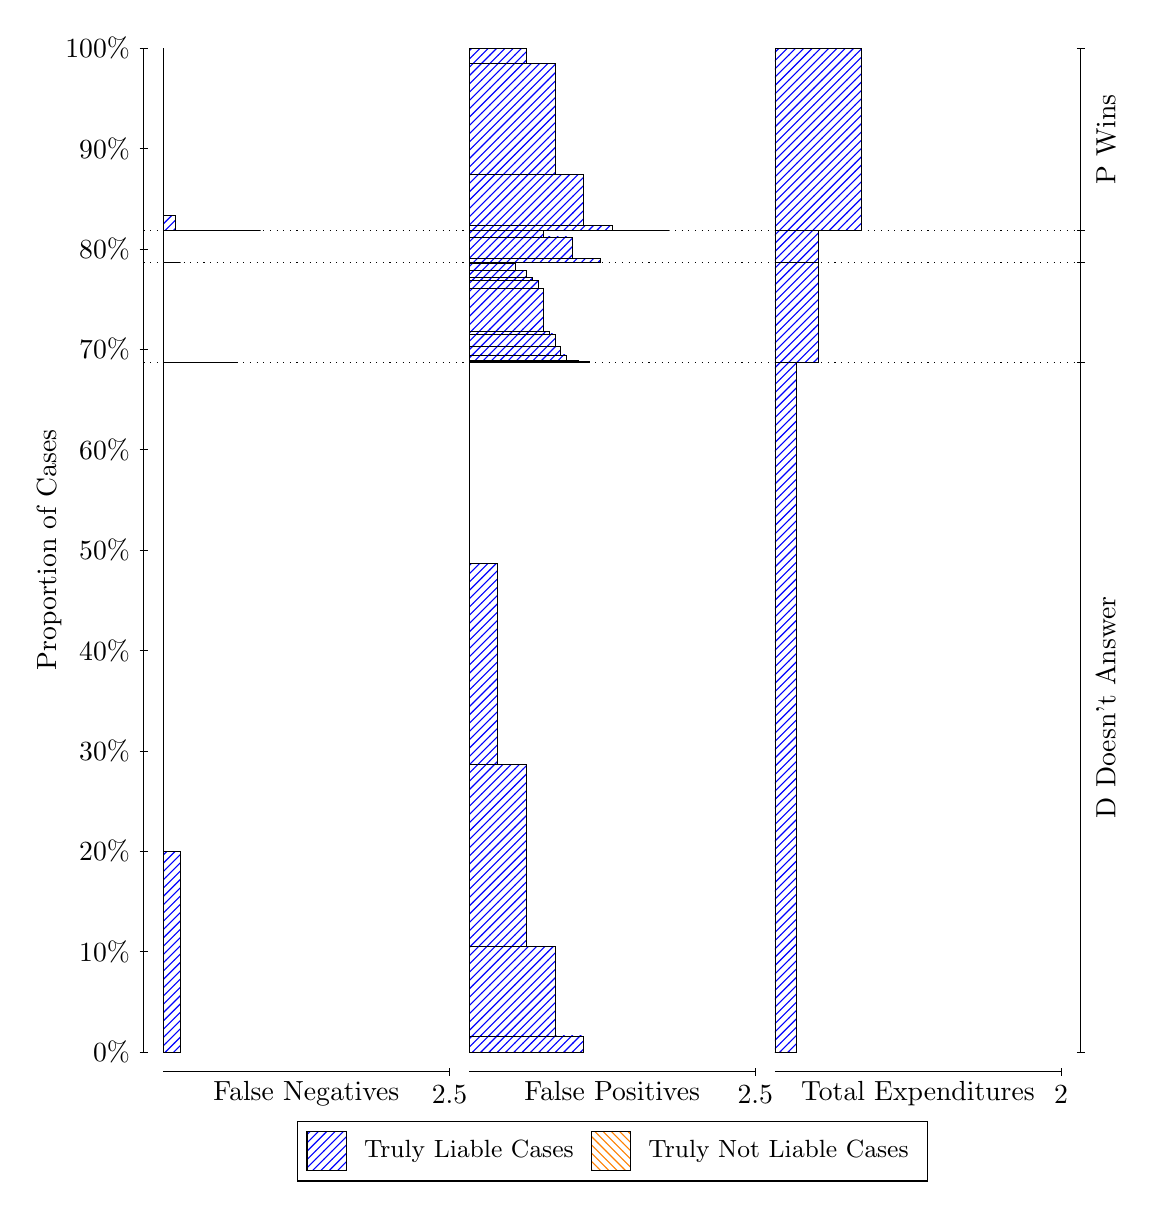
\begin{tikzpicture}
\draw[black, very thin] (1.5,1.75) -- (1.5,14.5);
\node[rotate=90, text=black, anchor=center] at (0.3, 8.125) {Proportion of Cases};
\draw[black, very thin] (1.45,1.75) -- (1.55,1.75);
\node[text=black, anchor=east] at (1.45, 1.75) {0\%};
\draw[black, very thin] (1.45,3.025) -- (1.55,3.025);
\node[text=black, anchor=east] at (1.45, 3.025) {10\%};
\draw[black, very thin] (1.45,4.3) -- (1.55,4.3);
\node[text=black, anchor=east] at (1.45, 4.3) {20\%};
\draw[black, very thin] (1.45,5.575) -- (1.55,5.575);
\node[text=black, anchor=east] at (1.45, 5.575) {30\%};
\draw[black, very thin] (1.45,6.85) -- (1.55,6.85);
\node[text=black, anchor=east] at (1.45, 6.85) {40\%};
\draw[black, very thin] (1.45,8.125) -- (1.55,8.125);
\node[text=black, anchor=east] at (1.45, 8.125) {50\%};
\draw[black, very thin] (1.45,9.4) -- (1.55,9.4);
\node[text=black, anchor=east] at (1.45, 9.4) {60\%};
\draw[black, very thin] (1.45,10.675) -- (1.55,10.675);
\node[text=black, anchor=east] at (1.45, 10.675) {70\%};
\draw[black, very thin] (1.45,11.95) -- (1.55,11.95);
\node[text=black, anchor=east] at (1.45, 11.95) {80\%};
\draw[black, very thin] (1.45,13.225) -- (1.55,13.225);
\node[text=black, anchor=east] at (1.45, 13.225) {90\%};
\draw[black, very thin] (1.45,14.5) -- (1.55,14.5);
\node[text=black, anchor=east] at (1.45, 14.5) {100\%};

\draw[black, very thin] (13.4,1.75) -- (13.4,14.5);
\draw[black, very thin] (13.35,1.75) -- (13.45,1.75);
\node[anchor=west] at (13.35, 1.75) {};
\draw[black, very thin] (13.35,10.505) -- (13.45,10.505);
\node[anchor=west] at (13.35, 10.505) {};
\draw[black, very thin] (13.35,11.774) -- (13.45,11.774);
\node[anchor=west] at (13.35, 11.774) {};
\draw[black, very thin] (13.35,12.181) -- (13.45,12.181);
\node[anchor=west] at (13.35, 12.181) {};
\draw[black, very thin] (13.35,14.5) -- (13.45,14.5);
\node[anchor=west] at (13.35, 14.5) {};

\draw[black, very thin, pattern color=blue, pattern=north east lines] (1.75,1.75) rectangle (1.968,4.2999);
\draw[black, very thin, pattern color=orange, pattern=north west lines] (1.75,4.2999) rectangle (1.75,4.2999);
\draw[black, very thin, pattern color=blue, pattern=north east lines] (1.75,4.2999) rectangle (1.75,10.505);
\draw[black, very thin, pattern color=blue, pattern=north east lines] (1.75,10.505) rectangle (2.6947,10.505);
\draw[black, very thin, pattern color=blue, pattern=north east lines] (1.75,10.505) rectangle (2.5493,10.505);
\draw[black, very thin, pattern color=blue, pattern=north east lines] (1.75,10.505) rectangle (2.404,10.505);
\draw[black, very thin, pattern color=blue, pattern=north east lines] (1.75,10.505) rectangle (2.3313,10.505);
\draw[black, very thin, pattern color=blue, pattern=north east lines] (1.75,10.505) rectangle (2.2587,10.505);
\draw[black, very thin, pattern color=blue, pattern=north east lines] (1.75,10.505) rectangle (2.186,10.505);
\draw[black, very thin, pattern color=blue, pattern=north east lines] (1.75,10.505) rectangle (2.1133,10.505);
\draw[black, very thin, pattern color=blue, pattern=north east lines] (1.75,10.505) rectangle (2.0407,10.505);
\draw[black, very thin, pattern color=blue, pattern=north east lines] (1.75,10.505) rectangle (1.968,10.507);
\draw[black, very thin, pattern color=blue, pattern=north east lines] (1.75,10.507) rectangle (1.8953,10.507);
\draw[black, very thin, pattern color=blue, pattern=north east lines] (1.75,10.507) rectangle (1.8227,10.509);
\draw[black, very thin, pattern color=orange, pattern=north west lines] (1.75,10.509) rectangle (1.75,10.509);
\draw[black, very thin, pattern color=blue, pattern=north east lines] (1.75,10.509) rectangle (1.75,11.774);
\draw[black, very thin, pattern color=blue, pattern=north east lines] (1.75,11.774) rectangle (1.968,11.774);
\draw[black, very thin, pattern color=orange, pattern=north west lines] (1.75,11.774) rectangle (1.75,11.774);
\draw[black, very thin, pattern color=blue, pattern=north east lines] (1.75,11.774) rectangle (1.75,12.181);
\draw[black, very thin, pattern color=blue, pattern=north east lines] (1.75,12.181) rectangle (2.9853,12.181);
\draw[black, very thin, pattern color=blue, pattern=north east lines] (1.75,12.181) rectangle (2.622,12.181);
\draw[black, very thin, pattern color=blue, pattern=north east lines] (1.75,12.181) rectangle (2.2587,12.181);
\draw[black, very thin, pattern color=blue, pattern=north east lines] (1.75,12.181) rectangle (2.2587,12.183);
\draw[black, very thin, pattern color=blue, pattern=north east lines] (1.75,12.183) rectangle (1.8953,12.184);
\draw[black, very thin, pattern color=blue, pattern=north east lines] (1.75,12.184) rectangle (1.8953,12.378);
\draw[black, very thin, pattern color=orange, pattern=north west lines] (1.75,12.378) rectangle (1.75,12.378);
\draw[black, very thin, pattern color=blue, pattern=north east lines] (1.75,12.378) rectangle (1.75,14.5);
\draw[black, very thin, pattern color=orange, pattern=north west lines] (5.6333,1.75) rectangle (7.0867,1.75);
\draw[black, very thin, pattern color=blue, pattern=north east lines] (5.6333,1.75) rectangle (7.0867,1.9546);
\draw[black, very thin, pattern color=blue, pattern=north east lines] (5.6333,1.9546) rectangle (6.7233,3.093);
\draw[black, very thin, pattern color=blue, pattern=north east lines] (5.6333,3.093) rectangle (6.36,5.4072);
\draw[black, very thin, pattern color=blue, pattern=north east lines] (5.6333,5.4072) rectangle (5.9967,7.9552);
\draw[black, very thin, pattern color=blue, pattern=north east lines] (5.6333,7.9552) rectangle (5.6333,10.505);
\draw[black, very thin, pattern color=orange, pattern=north west lines] (5.6333,10.505) rectangle (7.1593,10.505);
\draw[black, very thin, pattern color=blue, pattern=north east lines] (5.6333,10.505) rectangle (7.1593,10.523);
\draw[black, very thin, pattern color=orange, pattern=north west lines] (5.6333,10.523) rectangle (7.014,10.523);
\draw[black, very thin, pattern color=blue, pattern=north east lines] (5.6333,10.523) rectangle (7.014,10.53);
\draw[black, very thin, pattern color=orange, pattern=north west lines] (5.6333,10.53) rectangle (6.8687,10.53);
\draw[black, very thin, pattern color=blue, pattern=north east lines] (5.6333,10.53) rectangle (6.8687,10.603);
\draw[black, very thin, pattern color=blue, pattern=north east lines] (5.6333,10.603) rectangle (6.796,10.711);
\draw[black, very thin, pattern color=orange, pattern=north west lines] (5.6333,10.711) rectangle (6.7233,10.711);
\draw[black, very thin, pattern color=blue, pattern=north east lines] (5.6333,10.711) rectangle (6.7233,10.871);
\draw[black, very thin, pattern color=blue, pattern=north east lines] (5.6333,10.871) rectangle (6.6507,10.902);
\draw[black, very thin, pattern color=orange, pattern=north west lines] (5.6333,10.902) rectangle (6.578,10.902);
\draw[black, very thin, pattern color=blue, pattern=north east lines] (5.6333,10.902) rectangle (6.578,11.444);
\draw[black, very thin, pattern color=blue, pattern=north east lines] (5.6333,11.444) rectangle (6.5053,11.554);
\draw[black, very thin, pattern color=blue, pattern=north east lines] (5.6333,11.554) rectangle (6.4327,11.591);
\draw[black, very thin, pattern color=blue, pattern=north east lines] (5.6333,11.591) rectangle (6.36,11.672);
\draw[black, very thin, pattern color=blue, pattern=north east lines] (5.6333,11.672) rectangle (6.2873,11.674);
\draw[black, very thin, pattern color=blue, pattern=north east lines] (5.6333,11.674) rectangle (6.2147,11.765);
\draw[black, very thin, pattern color=blue, pattern=north east lines] (5.6333,11.765) rectangle (6.142,11.77);
\draw[black, very thin, pattern color=blue, pattern=north east lines] (5.6333,11.77) rectangle (6.0693,11.77);
\draw[black, very thin, pattern color=blue, pattern=north east lines] (5.6333,11.77) rectangle (5.9967,11.772);
\draw[black, very thin, pattern color=blue, pattern=north east lines] (5.6333,11.772) rectangle (5.924,11.772);
\draw[black, very thin, pattern color=blue, pattern=north east lines] (5.6333,11.772) rectangle (5.8513,11.774);
\draw[black, very thin, pattern color=blue, pattern=north east lines] (5.6333,11.774) rectangle (5.7787,11.774);
\draw[black, very thin, pattern color=blue, pattern=north east lines] (5.6333,11.774) rectangle (5.706,11.774);
\draw[black, very thin, pattern color=blue, pattern=north east lines] (5.6333,11.774) rectangle (5.6333,11.774);
\draw[black, very thin, pattern color=orange, pattern=north west lines] (5.6333,11.774) rectangle (7.3047,11.774);
\draw[black, very thin, pattern color=blue, pattern=north east lines] (5.6333,11.774) rectangle (7.3047,11.829);
\draw[black, very thin, pattern color=blue, pattern=north east lines] (5.6333,11.829) rectangle (6.9413,12.102);
\draw[black, very thin, pattern color=blue, pattern=north east lines] (5.6333,12.102) rectangle (6.578,12.18);
\draw[black, very thin, pattern color=blue, pattern=north east lines] (5.6333,12.18) rectangle (6.2147,12.181);
\draw[black, very thin, pattern color=blue, pattern=north east lines] (5.6333,12.181) rectangle (5.8513,12.181);
\draw[black, very thin, pattern color=orange, pattern=north west lines] (5.6333,12.181) rectangle (8.1767,12.181);
\draw[black, very thin, pattern color=blue, pattern=north east lines] (5.6333,12.181) rectangle (8.1767,12.181);
\draw[black, very thin, pattern color=orange, pattern=north west lines] (5.6333,12.181) rectangle (7.8133,12.181);
\draw[black, very thin, pattern color=blue, pattern=north east lines] (5.6333,12.181) rectangle (7.8133,12.182);
\draw[black, very thin, pattern color=orange, pattern=north west lines] (5.6333,12.182) rectangle (7.45,12.182);
\draw[black, very thin, pattern color=blue, pattern=north east lines] (5.6333,12.182) rectangle (7.45,12.245);
\draw[black, very thin, pattern color=orange, pattern=north west lines] (5.6333,12.245) rectangle (7.0867,12.245);
\draw[black, very thin, pattern color=blue, pattern=north east lines] (5.6333,12.245) rectangle (7.0867,12.898);
\draw[black, very thin, pattern color=orange, pattern=north west lines] (5.6333,12.898) rectangle (6.7233,12.898);
\draw[black, very thin, pattern color=blue, pattern=north east lines] (5.6333,12.898) rectangle (6.7233,14.303);
\draw[black, very thin, pattern color=blue, pattern=north east lines] (5.6333,14.303) rectangle (6.36,14.497);
\draw[black, very thin, pattern color=blue, pattern=north east lines] (5.6333,14.497) rectangle (5.9967,14.5);
\draw[black, very thin, pattern color=blue, pattern=north east lines] (5.6333,14.5) rectangle (5.6333,14.5);
\draw[black, very thin, pattern color=orange, pattern=north west lines] (9.5167,1.75) rectangle (9.7892,1.75);
\draw[black, very thin, pattern color=blue, pattern=north east lines] (9.5167,1.75) rectangle (9.7892,10.505);
\draw[black, very thin, pattern color=orange, pattern=north west lines] (9.5167,10.505) rectangle (10.062,10.505);
\draw[black, very thin, pattern color=blue, pattern=north east lines] (9.5167,10.505) rectangle (10.062,11.774);
\draw[black, very thin, pattern color=orange, pattern=north west lines] (9.5167,11.774) rectangle (10.062,11.774);
\draw[black, very thin, pattern color=blue, pattern=north east lines] (9.5167,11.774) rectangle (10.062,12.181);
\draw[black, very thin, pattern color=orange, pattern=north west lines] (9.5167,12.181) rectangle (10.607,12.181);
\draw[black, very thin, pattern color=blue, pattern=north east lines] (9.5167,12.181) rectangle (10.607,14.5);
\draw[black, dotted] (1.5,10.505) -- (13.4,10.505);
\draw[black, dotted] (1.5,11.774) -- (13.4,11.774);
\draw[black, dotted] (1.5,12.181) -- (13.4,12.181);
\draw[black, very thin] (1.75,1.5) -- (5.3833,1.5);
\node[text=black, anchor=north] at (3.5667, 1.5) {False Negatives};
\draw[black, very thin] (5.3833,1.45) -- (5.3833,1.55);
\node[text=black, anchor=north] at (5.3833, 1.45) {2.5};

\draw[black, very thin] (5.6333,1.5) -- (9.2667,1.5);
\node[text=black, anchor=north] at (7.45, 1.5) {False Positives};
\draw[black, very thin] (9.2667,1.45) -- (9.2667,1.55);
\node[text=black, anchor=north] at (9.2667, 1.45) {2.5};

\draw[black, very thin] (9.5167,1.5) -- (13.15,1.5);
\node[text=black, anchor=north] at (11.333, 1.5) {Total Expenditures};
\draw[black, very thin] (13.15,1.45) -- (13.15,1.55);
\node[text=black, anchor=north] at (13.15, 1.45) {2};

\node[text=black, centered, rotate=90] at (13.72, 6.1276) {D Doesn't Answer};


\node[text=black, centered, rotate=90] at (13.72, 13.34) {P Wins};

\draw (7.449999999999999,1.5) node[draw=none] (baseCoordinate) {};
\begin{scope}[align=center]
        \matrix[scale=0.5, draw=black, below=0.5cm of baseCoordinate, nodes={draw}, column sep=0.1cm]{
            \node[rectangle, draw, minimum width=0.5cm, minimum height=0.5cm, pattern color=blue, pattern=north east lines] {}; &
            \node[draw=none, font=\small, text=black] (B) {Truly Liable Cases}; &
            \node[rectangle, draw, minimum width=0.5cm, minimum height=0.5cm, pattern color=orange, pattern=north west lines] {}; &
            \node[draw=none, font=\small, text=black] (B) {Truly Not Liable Cases}; \\
            };
\end{scope}

\end{tikzpicture}
\end{document}